%%%%%%%%%%%%%%%%%%%%%%%%%%%%%%%%%%%%%%%%%%%%%%%%%%%%%%%%%%%
%                                                         %
%       This is documentation for the IPK project.        %
%                                                         %
%%%%%%%%%%%%%%%%%%%%%%%%%%%%%%%%%%%%%%%%%%%%%%%%%%%%%%%%%%%


%------------------------------------------------%
%	    CONFIGURATION + IMPORTED PACKAGES        %
%------------------------------------------------%
\documentclass[10pt,a4paper,titlepage]{article}
\usepackage[english]{babel}
\usepackage[utf8]{inputenc}
\usepackage[margin=100pt]{geometry}


\usepackage{graphicx}   % Import pictures
\usepackage{ragged2e}   % fullfill paragraphs
\usepackage{multicol}
\usepackage{lscape}

\newenvironment{changemargin}[2]{%
\begin{list}{}{%
\setlength{\topsep}{0pt}%
\setlength{\leftmargin}{#1}%
\setlength{\rightmargin}{#2}%
\setlength{\listparindent}{\parindent}%
\setlength{\itemindent}{\parindent}%
\setlength{\parsep}{\parskip}%
}%
\item[]}{\end{list}}

\begin{document}
%-----------------------------------------%
%	            TITLE PAGE                %
%-----------------------------------------%
\begin{titlepage}

\begin{center}
% Headings
\textsc{\LARGE Brno University of technology}\\[0.5cm]
\textsc{\large Faculty of Information Technology}\\[8cm]

% Title - lines
{ \huge \bfseries IPK project 1}\\[0.3cm]
{ \Large \bfseries documentation}\\[0.5cm]
{ \bfseries Martin Benes}\\

\end{center}

\end{titlepage}
\newpage

%-----------------------------------------%
%	              DOCUMENT                  %
%-----------------------------------------%

\setcounter{page}{1}
\pagenumbering{arabic}

\section{IPK project documentation}
The task was to create an client-server application in C/C++, that communicates
using BSD sockets and transfers files.

We ought to design our own protocol, that we use for the communication, and
describe it in documentation in detail.

\subsection{Protocol description}
I started with an analysis of BSD socket interface. Since it has semantics
as C, saving socket into buffer without being possible to reallocate the buffer,
I tried to deal with that in my design, so I would be able to save the data
using single function call into rightly sized buffer.

The protocol is built on TCP protocol, since it needs reliable transmission.


\begin{multicols}{2}
The protocol is described and implemented on two levels of abstraction,
the lower one enables sending and receiving byte, or string. Sending a
variably-sized data (strings) is preceded with sending a fixed-sized
({\it size\_t}) size of the data. That enables receiver to allocate a
buffer of the right size, so the data fits in.

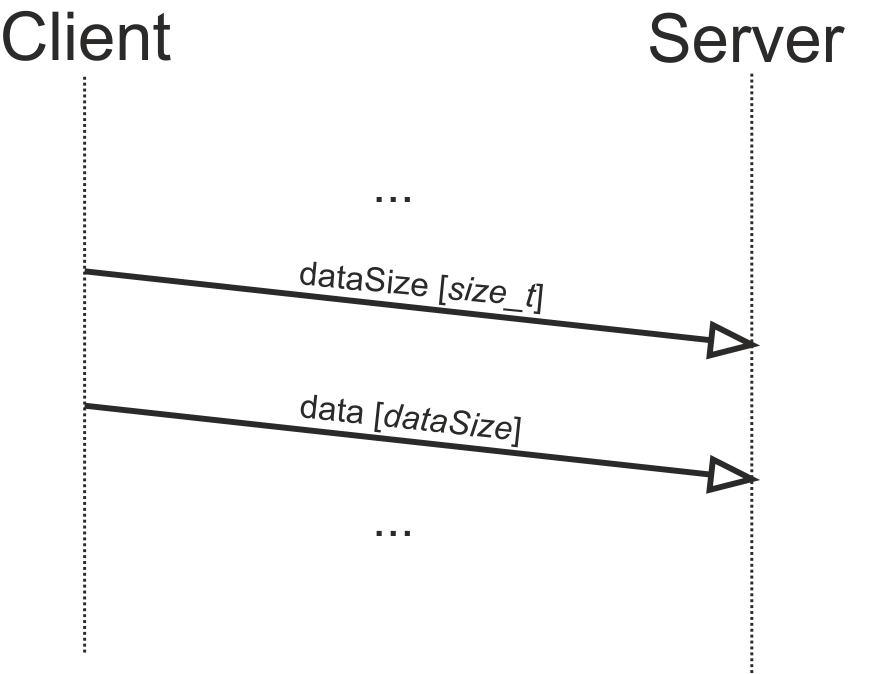
\includegraphics[width=0.37\textwidth]{send_data.png}
\end{multicols}


\begin{multicols}{2}
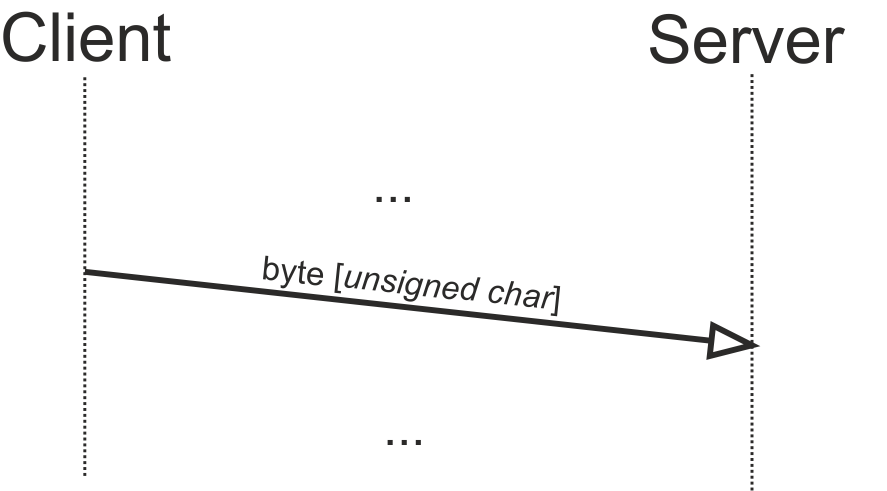
\includegraphics[width=0.4\textwidth]{send_byte.png}

The protocol may send a single byte too. It is used to send an indication
to the opposite side, such as errors etc. For example, the client sends
the mode (read/write), or server announces if the reading of file succeeded.

In this case, the sent data is fixed-sized ({\it unsigned~char}),
so it does not have to do the same routine as the above mentioned.
\end{multicols}

The higher abstraction layer (the program itself) uses the services
of the lower. For simplification of the images, the sending of the size
of data will not be displayed.

The server is listening on the port and the client is connecting
to the server with explicitly given address and port. The mode
of usage (read/write) is also given.


\begin{multicols}{2}
The read is initiated, when argument {\it -r} is given, following with
a {\it path}. The first to send as a client is a byte 0xFF, that means
the reading mode is selected.

The second thing to send is the {\it full path of file}. Afterwards, the {\it file}
itself is expected to receive from the server in the form of string.

The semantics of sending a string are used here, as same as during the sending
of a file path.

When the file data arrives, they are written into the file of the same name,
as the received one.

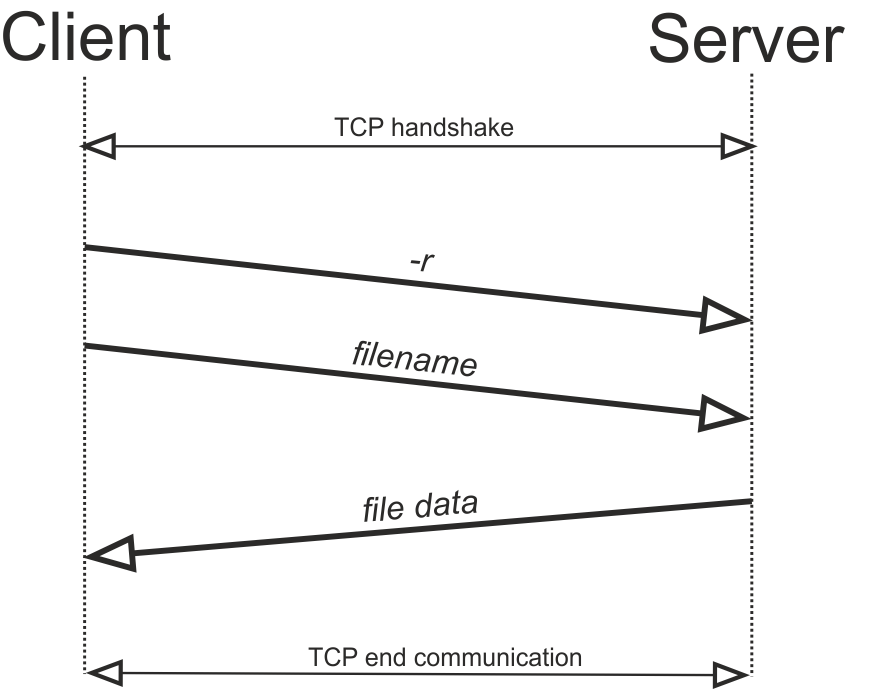
\includegraphics[width=0.5\textwidth]{read.png}
\end{multicols}


\begin{multicols}{2}
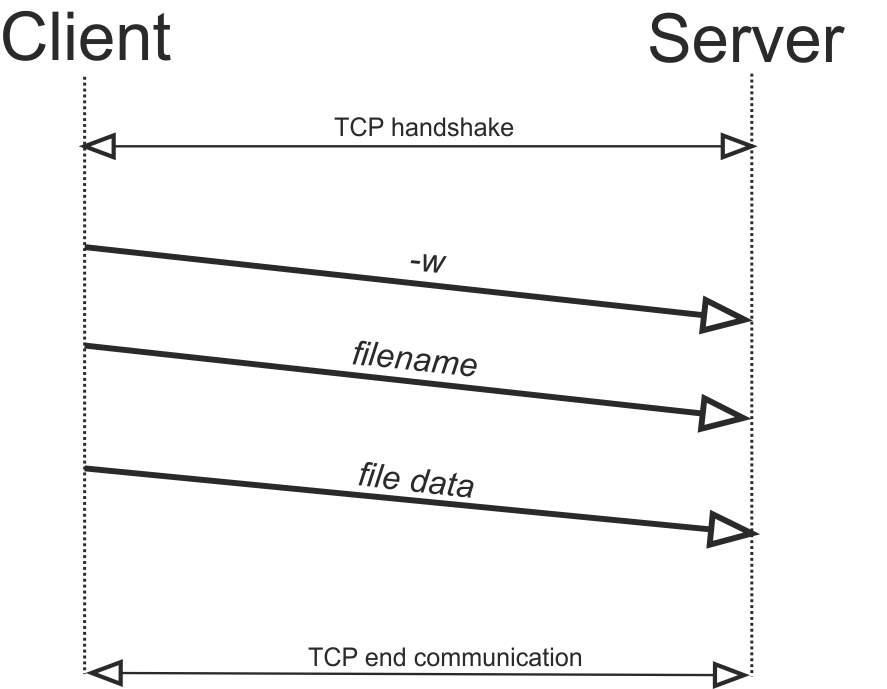
\includegraphics[width=0.5\textwidth]{write.png}

The write is similar as read with slight differences, it is initialized
with a given argument {\it -w} and the {\it path} afterwards. The first byte
is 0x00, indicating the write mode.

Then the client sends {\it the name of the file} (without the path), on the
server, it will be located in the working directory.

The client follows with sending {\it the file data}. Again, it is done
with the mentioned method of sending variably-sized strings.

The server then writes the received data to the file.

\end{multicols}

\subsection{Implementation}

The lower level of protocol is implemented as class hierarchy, so it is
encapsulated and may be instatiated. There is an abstract class {\it Socket},
which contains common code for both client and server, and inherited
{\it ClientSocket} and {\it ServerSocket}, that implements the distinct parts.
They also covers the BDS socket interface calling, so basically only these
classes is directly dependent on BSD socket interface.

There are two programs, {\it ipk-server} and {\it ipk-client}, each has its
own module, {\it server.cpp} and {\it client.cpp}. They contain implementation
of higher-abstraction level of my protocol, as described above.

The server is concurrent, using {\it fork()} call and utilities from
{\it signal.h} standard C library, which means it can operate with multiple
clients at one time.

There are also some common moduls used by both of the programs: {\it config.h},
{\it defs.h} and {\it mysocket.h}. The module {\it config.h} defines
{\it Config} class, which is used to process arguments, to check if they are
valid for the program it is used in and to hold the configuration of the program.
The module {\it defs.h} includes debug constants and common functions.

The module {\it mysocket.h} contains the {\it Socket} class definition, as well
as the inherited classes, {\it ClientSocket} and {\it ServerSocket}. It
provides an interface, that is then well legible at the {\it client.cpp}
and {\it server.cpp} modules, where it is used.



\end{document}
